\documentclass{article}


% if you need to pass options to natbib, use, e.g.:
%     \PassOptionsToPackage{numbers, compress}{natbib}
% before loading neurips_2022


% ready for submission
\usepackage[preprint]{neurips_2022}


% to compile a preprint version, e.g., for submission to arXiv, add add the
% [preprint] option:
%     \usepackage[preprint]{neurips_2022}


% to compile a camera-ready version, add the [final] option, e.g.:
%     \usepackage[final]{neurips_2022}


% to avoid loading the natbib package, add option nonatbib:
%    \usepackage[nonatbib]{neurips_2022}


\usepackage[utf8]{inputenc} % allow utf-8 input
\usepackage[T1]{fontenc}    % use 8-bit T1 fonts
\usepackage{hyperref}       % hyperlinks
\usepackage{url}            % simple URL typesetting
\usepackage{booktabs}       % professional-quality tables
\usepackage{amsfonts}       % blackboard math symbols
\usepackage{nicefrac}       % compact symbols for 1/2, etc.
\usepackage{microtype}      % microtypography
\usepackage{xcolor}         % colors

% Felix's packages
\usepackage{amsmath}
\usepackage{amssymb}
\usepackage[shortlabels]{enumitem}
\usepackage{mathtools}
\usepackage{mathrsfs}
\usepackage{dsfont}
\usepackage{physics}
\usepackage{caption}
\usepackage{subcaption}
\usepackage[nameinlink]{cleveref}

% floor, ceiling, set
\DeclarePairedDelimiter{\ceil}{\lceil}{\rceil}
\DeclarePairedDelimiter{\floor}{\lfloor}{\rfloor}
\DeclarePairedDelimiter{\set}{\lbrace}{\rbrace}
\DeclarePairedDelimiter{\iprod}{\langle}{\rangle}
\DeclarePairedDelimiter{\card}{\lvert}{\rvert}
\let\abs\relax
\DeclarePairedDelimiter{\abs}{\lvert}{\rvert}
\DeclarePairedDelimiter{\level}{\llbracket}{\rrbracket}

\DeclareMathOperator{\Int}{int}
\DeclareMathOperator{\bdy}{bdy}
\DeclareMathOperator{\Lim}{Lim}
\DeclareMathOperator{\mean}{mean}
\DeclareMathOperator{\col}{col}
\DeclareMathOperator{\proj}{proj}
\DeclareMathOperator{\dual}{dual}
\usepackage[nameinlink]{cleveref}
\DeclareMathOperator{\opt}{opt}
\DeclareMathOperator{\cone}{cone}
\DeclareMathOperator{\conv}{conv}
\DeclareMathOperator{\supp}{supp}
\DeclareMathOperator{\poly}{poly}
\DeclareMathOperator{\sgn}{sgn}
\DeclareMathOperator{\depth}{depth}
\DeclareMathOperator{\OPT}{OPT}
\DeclareMathOperator{\Set}{set}
\DeclareMathOperator{\pred}{pred}
\DeclareMathOperator{\SAT}{SAT}
\DeclareMathOperator{\indeg}{indeg}
\DeclareMathOperator{\outdeg}{outdeg}
\DeclareMathOperator{\tw}{tw}
\DeclareMathOperator{\bw}{bw}
\DeclareMathOperator{\pw}{pw}
\DeclareMathOperator{\cutwidth}{cutwidth}
\DeclareMathOperator{\Cut}{Cut}
\DeclareMathOperator{\Vs}{Vs}
\DeclareMathOperator{\vs}{vs}
\DeclareMathOperator{\adj}{adj}
\DeclareMathOperator{\Sp}{Sp}
\DeclareMathOperator{\argmax}{argmax}
\DeclareMathOperator{\argmin}{argmin}
\DeclareMathOperator{\dom}{dom}
\DeclareMathOperator{\MLE}{MLE}
\DeclareMathOperator{\MAP}{MAP}
\DeclareMathOperator{\KL}{KL}
\DeclareMathOperator{\LK}{LK}
\DeclareMathOperator{\Be}{Be}
\DeclareMathOperator{\Bin}{Bin}
\DeclareMathOperator{\Geo}{Geo}
\DeclareMathOperator{\Po}{Po}
\DeclareMathOperator{\Exp}{Exp}
\DeclareMathOperator{\Mult}{Mult}
\DeclareMathOperator{\Var}{Var}
\DeclareMathOperator{\Cov}{Cov}
\DeclareMathOperator{\Cauchy}{Cauchy}

% commonly used sets
\newcommand{\R}{\mathbb{R}}
\newcommand{\Z}{\mathbb{Z}}
\newcommand{\N}{\mathbb{N}}
\newcommand{\Q}{\mathbb{Q}}
\newcommand{\C}{\mathbb{C}}
\newcommand{\E}{\mathbb{E}}
\newcommand{\B}{\mathcal{B}}
\newcommand{\F}{\mathcal{F}}
\renewcommand{\L}{\mathcal{L}}
\renewcommand{\P}{\mathbb{P}}

\newcommand{\sset}{\subseteq}
\newcommand{\mcal}{\mathcal}
\newcommand{\mscr}{\mathscr}
\newcommand{\mfrak}{\mathfrak}
\newcommand{\up}{\uparrow}
\newcommand{\down}{\downarrow}
\newcommand{\zeros}{\mathds{0}}
\newcommand{\ones}{\mathds{1}}
\newcommand{\tends}[1]{\xrightarrow{#1}}

\newcommand{\Partition}{{\sc Partition}}

\renewcommand{\bibsection}{}


\title{Weighted Maximum Independent Set Heuristics with Graph Neural Networks}


% The \author macro works with any number of authors. There are two commands
% used to separate the names and addresses of multiple authors: \And and \AND.
%
% Using \And between authors leaves it to LaTeX to determine where to break the
% lines. Using \AND forces a line break at that point. So, if LaTeX puts 3 of 4
% authors names on the first line, and the last on the second line, try using
% \AND instead of \And before the third author name.


\author{%
  Felix Zhou\\
  Department of Computer Science\\
  Yale University\\
  New Haven, CT 06511 \\
  \texttt{felix.zhou@yale.edu} \\
  % examples of more authors
  % \And
  % Coauthor \\
  % Affiliation \\
  % Address \\
  % \texttt{email} \\
  % \AND
  % Coauthor \\
  % Affiliation \\
  % Address \\
  % \texttt{email} \\
  % \And
  % Coauthor \\
  % Affiliation \\
  % Address \\
  % \texttt{email} \\
  % \And
  % Coauthor \\
  % Affiliation \\
  % Address \\
  % \texttt{email} \\
}


\begin{document}


\maketitle


\begin{abstract}
  The weighted maximum indepedent set (WMIS) problem asks us to find a subset of pairwise non-adjacent vertices
  which maximizes the sum of vertex weights.
  In general, there cannot be a constant factor polynomial time approximation algorithm.
  In theory, much progress has been made for solving WMIS for special classes of graphs.
  In practice, exact algorithms based on reduction rules and branching techniques have been examined
  in conjunction with search-based heuristics.
  Graph neural networks (GNNs) have been shown to be effective at learning the structure of real-world graphs.
  Recent efforts have been made to combine simple GNNs with exact methods and iterative search.
  We analyze the performance of different GNN architectures within this paradigm.
  We also provide an easily extensible python implementation of our algorithms for futher exploration.
\end{abstract}


\section{Introduction \& Problem Definition}
Let $G=(V, E)$ be a (simple, undirected) graph with vertex set $V$
and edge set $E$.
Suppose we also have vertex sets $w: V\to \R_{++}$.
Recall that a subset of vertices $I\sset V$ is \emph{independent}
if for every $u\neq v\in I$, $uv\notin E$.
That is, the vertices in $I$ are pairwise non-adjacent.
The weighted maximum independent set problem (WMIS)
asks us to find an independent set $I$ which maximizes
\[
  w(I) := \sum_{v\in I} w(v).
\]
Note that $I$ is a WMIS in $G$
if and only if $V\setminus I$ is a weighted minimum vertex cover (WMVC) in $G$.
The unweighted decision version of the minimum vertex cover problem (MVC)
was one of Karp's original 21 NP-complete problems.
It follows that both WMVC and WMIS are both NP-hard.
In general graphs,
it is known that the independent set problem (MIS) cannot be approximated within a factor of $n^{1-\epsilon}$ for any $\epsilon > 0$ where $n$ is the number of vertices \citet{zuckerman2006linear}.
In fact, even in 3-regular 3-edge-colorable graphs,
there can be no polynomial time approximation scheme (PTAS) \citet{berman1999appr}.

It is helpful to think of WMIS as a 0-1 integer program.
\begin{align*}
  &\max \sum_{v\in V} w(v) x(v) \\
  x(u) + x(v) &\leq 1 &&\forall uv\in E \\
  x &\in \set{0, 1}
\end{align*}
Although we cannot hope to solve 0-1 integer programs polynomial time,
we can relax the integral constraints to form a linear program.
\begin{align*}
  &\max \sum_{v\in V} w(v) x(v) \\
  x(u) + x(v) &\leq 1 &&\forall uv\in E \\
  x &\geq 0 \\
  x &\leq 1
\end{align*}
Solving this linear program yields a solution $\bar x\in [0, 1]^n$.
It is known that if $\bar x(v) = 1$,
then there is a WMIS which includes $v$
and if $\bar x(v) = 0$,
then there is a WMIS which does not include $v$ \citet{lpreduction}.
Thus we can shrink an instance of WMIS by first solving a linear program
and enforcing that integral vertices are (not) part of the solution.
This is an example of a reduction rule which reduces the sizes of instances
such that any optimal solution for the reduced instance can be expanded to an optimal solution
for the original solution.

Practical solvers for WMIS extensively use reduction rules
in hopes that we can significantly reduce instances
before applying brute force or a heuristic search \cite{kamis}.
\citet{langedal_et_al} proposed a hybrid approach
which uses reductions, a graph neural network (GNN), and a solver to compute an initial feasible solution.
This is solution is then improved using iterative search.

\section{Dataset}
We consider both real-world graphs and synthetic graphs.
Since these graphs do not come with weights,
we augment each instance with uniformly random integer weights within the interval $[1, N]$.
It is known that with probability at least $1-\frac nN$,
there is a unique solution to WMIS \citet{isolation}.
Thus we chose $N = 2n$ in hopes that this disambiguates supervised learning.

\subsection{PACE 2019 Graphs}
The PACE 2019 competition asked participants to solve MVC in 200 real-world graphs \citet{pace2019}.
Half of the dataset was provided to contestants and the remaining half was used to evaluate submissions.
Solvers were given 30 minutes to solve each instance exactly.

For each of the 200 graphs, we sampled 100 instances of uniform random weights.
Out of the 10000 instances,  
the state-of-the-art branch and reduce (B\&R) solver by \citet{kamis} solved 18197 cases within 6 hours.

See \Cref{fig:pace} for some elementary statistics about the pace dataset.
It is interesting to note that this dataset is relatively sparse,
with mostly single digit average degree.
Moreover, most graphs have very few connected components.

\begin{figure}
     \centering
     \begin{subfigure}[b]{0.45\textwidth}
         \centering
         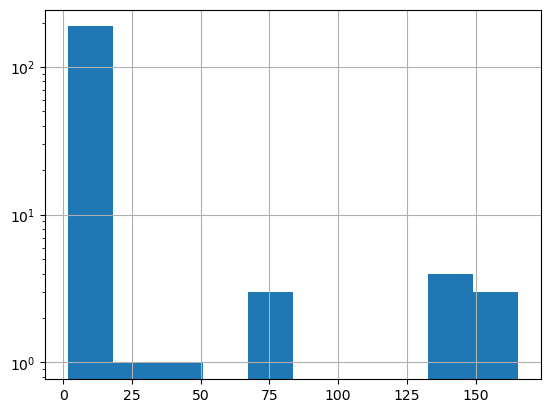
\includegraphics[width=\textwidth]{figures/pace_avg_deg}
         \caption{Average degree of pace graphs.}
         \label{fig:pace_avg_deg}
     \end{subfigure}
     \hfill
     \begin{subfigure}[b]{0.45\textwidth}
         \centering
         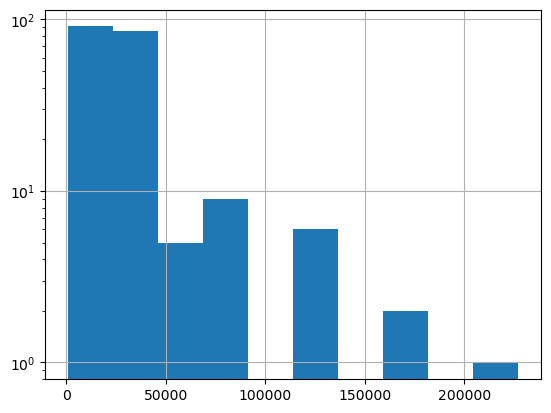
\includegraphics[width=\textwidth]{figures/pace_n_nodes}
         \caption{Number of nodes in pace graphs.}
         \label{fig:pace_n_nodes}
     \end{subfigure}
     
     \bigskip
     \begin{subfigure}[b]{0.45\textwidth}
         \centering
         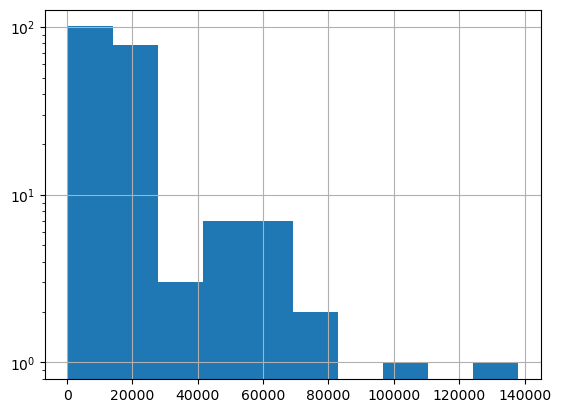
\includegraphics[width=\textwidth]{figures/pace_n_edges}
         \caption{number of edges in pace graphs.}
         \label{fig:pace_n_edges}
     \end{subfigure}
     \hfill
     \begin{subfigure}[b]{0.45\textwidth}
         \centering
         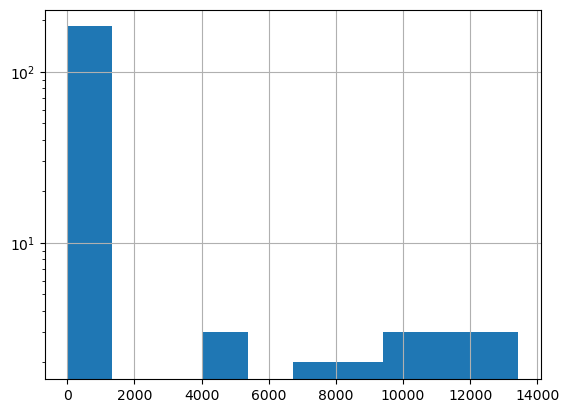
\includegraphics[width=\textwidth]{figures/pace_n_components}
         \caption{Number of components in pace graphs.}
         \label{fig:pace_n_components}
     \end{subfigure}
     \caption{Basic graph statistics as histograms for pace graphs.}
     \label{fig:pace}
\end{figure}

\subsection{Erd\H os-R\'eyni Graphs}
We can generate an instance of an Erd\H os-R\'eyni graph $G(n, p)$ on $n$ vertices
by randomly connecting every pair of vertices independently
with some fixed probability $p$.
Since these are very well-studied graphs,
we omit the graph statistics.

We generated 1000 instaces of $G(200, 0.1)$,
for which the B\&R solver by \citet{kamis} solved all cases within 6 hours.
Next, we generate 5000 instances of $G(1000, 0.005)$,
for which the B\&R solver solved 400 cases within 6 hours.
Finally, we generated 20000 instances of $G(50000, 0.00005)$.
for which the B\&R solver solved all cases within 6 hours.

\subsection{Watts-Strogatz Graphs}
If time permits, we would also like to experiment with Watts-Strogatz graphs.
Also called ``small-world graphs'',
these graphs are generated by first taking a $k$-regular graph
and randomly reassigning the endpoints of edges to other vertices.

\section{Description of Related Works}
Efficient Minimum Weight Vertex Cover Heuristics Using Graph Neural Networks by \citet{langedal_et_al}.

SuiteSparse graphs \citet{suitesparse}.

KaMIS weighted branch and reduce algorithm by \citet{kamis}.

WeGotYouCovered solver by \citet{wegotyoucovered}.

Reducing peeling with GCNs by \citet{comboptgcn}.

\section{Proposed Approaches}
Identity-Aware GNN by \citet{idgnn}.

Graph convolutional network by \citet{gcn}.

Pytorch framework by \citet{pytorch}.

Pytorch geometric by \citet{pyg}.

Gurobi solver by \citet{gurobi}.

LP based reduction by \citet{lpreduction}.

\section{Evaluation Metrics}
\section{Timeline}
\section{References}
\bibliographystyle{plainnat}
\bibliography{proposal.bib}

\clearpage
\section{Submission of papers to NeurIPS 2022}


Please read the instructions below carefully and follow them faithfully.


\subsection{Style}


Papers to be submitted to NeurIPS 2022 must be prepared according to the
instructions presented here. Papers may only be up to {\bf nine} pages long,
including figures. Additional pages \emph{containing only acknowledgments and
references} are allowed. Papers that exceed the page limit will not be
reviewed, or in any other way considered for presentation at the conference.


The margins in 2022 are the same as those in 2007, which allow for $\sim$$15\%$
more words in the paper compared to earlier years.


Authors are required to use the NeurIPS \LaTeX{} style files obtainable at the
NeurIPS website as indicated below. Please make sure you use the current files
and not previous versions. Tweaking the style files may be grounds for
rejection.


\subsection{Retrieval of style files}


The style files for NeurIPS and other conference information are available on
the World Wide Web at
\begin{center}
  \url{http://www.neurips.cc/}
\end{center}
The file \verb+neurips_2022.pdf+ contains these instructions and illustrates the
various formatting requirements your NeurIPS paper must satisfy.


The only supported style file for NeurIPS 2022 is \verb+neurips_2022.sty+,
rewritten for \LaTeXe{}.  \textbf{Previous style files for \LaTeX{} 2.09,
  Microsoft Word, and RTF are no longer supported!}


The \LaTeX{} style file contains three optional arguments: \verb+final+, which
creates a camera-ready copy, \verb+preprint+, which creates a preprint for
submission to, e.g., arXiv, and \verb+nonatbib+, which will not load the
\verb+natbib+ package for you in case of package clash.


\paragraph{Preprint option}
If you wish to post a preprint of your work online, e.g., on arXiv, using the
NeurIPS style, please use the \verb+preprint+ option. This will create a
nonanonymized version of your work with the text ``Preprint. Work in progress.''
in the footer. This version may be distributed as you see fit. Please \textbf{do
  not} use the \verb+final+ option, which should \textbf{only} be used for
papers accepted to NeurIPS.


At submission time, please omit the \verb+final+ and \verb+preprint+
options. This will anonymize your submission and add line numbers to aid
review. Please do \emph{not} refer to these line numbers in your paper as they
will be removed during generation of camera-ready copies.


The file \verb+neurips_2022.tex+ may be used as a ``shell'' for writing your
paper. All you have to do is replace the author, title, abstract, and text of
the paper with your own.


The formatting instructions contained in these style files are summarized in
Sections \ref{gen_inst}, \ref{headings}, and \ref{others} below.


\section{General formatting instructions}
\label{gen_inst}


The text must be confined within a rectangle 5.5~inches (33~picas) wide and
9~inches (54~picas) long. The left margin is 1.5~inch (9~picas).  Use 10~point
type with a vertical spacing (leading) of 11~points.  Times New Roman is the
preferred typeface throughout, and will be selected for you by default.
Paragraphs are separated by \nicefrac{1}{2}~line space (5.5 points), with no
indentation.


The paper title should be 17~point, initial caps/lower case, bold, centered
between two horizontal rules. The top rule should be 4~points thick and the
bottom rule should be 1~point thick. Allow \nicefrac{1}{4}~inch space above and
below the title to rules. All pages should start at 1~inch (6~picas) from the
top of the page.


For the final version, authors' names are set in boldface, and each name is
centered above the corresponding address. The lead author's name is to be listed
first (left-most), and the co-authors' names (if different address) are set to
follow. If there is only one co-author, list both author and co-author side by
side.


Please pay special attention to the instructions in Section \ref{others}
regarding figures, tables, acknowledgments, and references.


\section{Headings: first level}
\label{headings}


All headings should be lower case (except for first word and proper nouns),
flush left, and bold.


First-level headings should be in 12-point type.


\subsection{Headings: second level}


Second-level headings should be in 10-point type.


\subsubsection{Headings: third level}


Third-level headings should be in 10-point type.


\paragraph{Paragraphs}


There is also a \verb+\paragraph+ command available, which sets the heading in
bold, flush left, and inline with the text, with the heading followed by 1\,em
of space.


\section{Citations, figures, tables, references}
\label{others}


These instructions apply to everyone.


\subsection{Citations within the text}


The \verb+natbib+ package will be loaded for you by default.  Citations may be
author/year or numeric, as long as you maintain internal consistency.  As to the
format of the references themselves, any style is acceptable as long as it is
used consistently.


The documentation for \verb+natbib+ may be found at
\begin{center}
  \url{http://mirrors.ctan.org/macros/latex/contrib/natbib/natnotes.pdf}
\end{center}
Of note is the command \verb+\citet+, which produces citations appropriate for
use in inline text.  For example,
\begin{verbatim}
   \citet{hasselmo} investigated\dots
\end{verbatim}
produces
\begin{quote}
  Hasselmo, et al.\ (1995) investigated\dots
\end{quote}


If you wish to load the \verb+natbib+ package with options, you may add the
following before loading the \verb+neurips_2022+ package:
\begin{verbatim}
   \PassOptionsToPackage{options}{natbib}
\end{verbatim}


If \verb+natbib+ clashes with another package you load, you can add the optional
argument \verb+nonatbib+ when loading the style file:
\begin{verbatim}
   \usepackage[nonatbib]{neurips_2022}
\end{verbatim}


As submission is double blind, refer to your own published work in the third
person. That is, use ``In the previous work of Jones et al.\ [4],'' not ``In our
previous work [4].'' If you cite your other papers that are not widely available
(e.g., a journal paper under review), use anonymous author names in the
citation, e.g., an author of the form ``A.\ Anonymous.''


\subsection{Footnotes}


Footnotes should be used sparingly.  If you do require a footnote, indicate
footnotes with a number\footnote{Sample of the first footnote.} in the
text. Place the footnotes at the bottom of the page on which they appear.
Precede the footnote with a horizontal rule of 2~inches (12~picas).


Note that footnotes are properly typeset \emph{after} punctuation
marks.\footnote{As in this example.}


\subsection{Figures}


\begin{figure}
  \centering
  \fbox{\rule[-.5cm]{0cm}{4cm} \rule[-.5cm]{4cm}{0cm}}
  \caption{Sample figure caption.}
\end{figure}


All artwork must be neat, clean, and legible. Lines should be dark enough for
purposes of reproduction. The figure number and caption always appear after the
figure. Place one line space before the figure caption and one line space after
the figure. The figure caption should be lower case (except for first word and
proper nouns); figures are numbered consecutively.


You may use color figures.  However, it is best for the figure captions and the
paper body to be legible if the paper is printed in either black/white or in
color.


\subsection{Tables}


All tables must be centered, neat, clean and legible.  The table number and
title always appear before the table.  See Table~\ref{sample-table}.


Place one line space before the table title, one line space after the
table title, and one line space after the table. The table title must
be lower case (except for first word and proper nouns); tables are
numbered consecutively.


Note that publication-quality tables \emph{do not contain vertical rules.} We
strongly suggest the use of the \verb+booktabs+ package, which allows for
typesetting high-quality, professional tables:
\begin{center}
  \url{https://www.ctan.org/pkg/booktabs}
\end{center}
This package was used to typeset Table~\ref{sample-table}.


\begin{table}
  \caption{Sample table title}
  \label{sample-table}
  \centering
  \begin{tabular}{lll}
    \toprule
    \multicolumn{2}{c}{Part}                   \\
    \cmidrule(r){1-2}
    Name     & Description     & Size ($\mu$m) \\
    \midrule
    Dendrite & Input terminal  & $\sim$100     \\
    Axon     & Output terminal & $\sim$10      \\
    Soma     & Cell body       & up to $10^6$  \\
    \bottomrule
  \end{tabular}
\end{table}


\section{Final instructions}


Do not change any aspects of the formatting parameters in the style files.  In
particular, do not modify the width or length of the rectangle the text should
fit into, and do not change font sizes (except perhaps in the
\textbf{References} section; see below). Please note that pages should be
numbered.


\section{Preparing PDF files}


Please prepare submission files with paper size ``US Letter,'' and not, for
example, ``A4.''


Fonts were the main cause of problems in the past years. Your PDF file must only
contain Type 1 or Embedded TrueType fonts. Here are a few instructions to
achieve this.


\begin{itemize}


\item You should directly generate PDF files using \verb+pdflatex+.


\item You can check which fonts a PDF files uses.  In Acrobat Reader, select the
  menu Files$>$Document Properties$>$Fonts and select Show All Fonts. You can
  also use the program \verb+pdffonts+ which comes with \verb+xpdf+ and is
  available out-of-the-box on most Linux machines.


\item The IEEE has recommendations for generating PDF files whose fonts are also
  acceptable for NeurIPS. Please see
  \url{http://www.emfield.org/icuwb2010/downloads/IEEE-PDF-SpecV32.pdf}


\item \verb+xfig+ "patterned" shapes are implemented with bitmap fonts.  Use
  "solid" shapes instead.


\item The \verb+\bbold+ package almost always uses bitmap fonts.  You should use
  the equivalent AMS Fonts:
\begin{verbatim}
   \usepackage{amsfonts}
\end{verbatim}
followed by, e.g., \verb+\mathbb{R}+, \verb+\mathbb{N}+, or \verb+\mathbb{C}+
for $\mathbb{R}$, $\mathbb{N}$ or $\mathbb{C}$.  You can also use the following
workaround for reals, natural and complex:
\begin{verbatim}
   \newcommand{\RR}{I\!\!R} %real numbers
   \newcommand{\Nat}{I\!\!N} %natural numbers
   \newcommand{\CC}{I\!\!\!\!C} %complex numbers
\end{verbatim}
Note that \verb+amsfonts+ is automatically loaded by the \verb+amssymb+ package.


\end{itemize}


If your file contains type 3 fonts or non embedded TrueType fonts, we will ask
you to fix it.


\subsection{Margins in \LaTeX{}}


Most of the margin problems come from figures positioned by hand using
\verb+\special+ or other commands. We suggest using the command
\verb+\includegraphics+ from the \verb+graphicx+ package. Always specify the
figure width as a multiple of the line width as in the example below:
\begin{verbatim}
   \usepackage[pdftex]{graphicx} ...
   \includegraphics[width=0.8\linewidth]{myfile.pdf}
\end{verbatim}
See Section 4.4 in the graphics bundle documentation
(\url{http://mirrors.ctan.org/macros/latex/required/graphics/grfguide.pdf})


A number of width problems arise when \LaTeX{} cannot properly hyphenate a
line. Please give LaTeX hyphenation hints using the \verb+\-+ command when
necessary.


\begin{ack}
Use unnumbered first level headings for the acknowledgments. All acknowledgments
go at the end of the paper before the list of references. Moreover, you are required to declare
funding (financial activities supporting the submitted work) and competing interests (related financial activities outside the submitted work).
More information about this disclosure can be found at: \url{https://neurips.cc/Conferences/2022/PaperInformation/FundingDisclosure}.


Do {\bf not} include this section in the anonymized submission, only in the final paper. You can use the \texttt{ack} environment provided in the style file to autmoatically hide this section in the anonymized submission.
\end{ack}


\section{References}

References follow the acknowledgments. Use unnumbered first-level heading for
the references. Any choice of citation style is acceptable as long as you are
consistent. It is permissible to reduce the font size to \verb+small+ (9 point)
when listing the references.
Note that the Reference section does not count towards the page limit.

%%%%%%%%%%%%%%%%%%%%%%%%%%%%%%%%%%%%%%%%%%%%%%%%%%%%%%%%%%%%
\section*{Checklist}


%%% BEGIN INSTRUCTIONS %%%
The checklist follows the references.  Please
read the checklist guidelines carefully for information on how to answer these
questions.  For each question, change the default \answerTODO{} to \answerYes{},
\answerNo{}, or \answerNA{}.  You are strongly encouraged to include a {\bf
justification to your answer}, either by referencing the appropriate section of
your paper or providing a brief inline description.  For example:
\begin{itemize}
  \item Did you include the license to the code and datasets? \answerYes{See Section~\ref{gen_inst}.}
  \item Did you include the license to the code and datasets? \answerNo{The code and the data are proprietary.}
  \item Did you include the license to the code and datasets? \answerNA{}
\end{itemize}
Please do not modify the questions and only use the provided macros for your
answers.  Note that the Checklist section does not count towards the page
limit.  In your paper, please delete this instructions block and only keep the
Checklist section heading above along with the questions/answers below.
%%% END INSTRUCTIONS %%%


\begin{enumerate}


\item For all authors...
\begin{enumerate}
  \item Do the main claims made in the abstract and introduction accurately reflect the paper's contributions and scope?
    \answerTODO{}
  \item Did you describe the limitations of your work?
    \answerTODO{}
  \item Did you discuss any potential negative societal impacts of your work?
    \answerTODO{}
  \item Have you read the ethics review guidelines and ensured that your paper conforms to them?
    \answerTODO{}
\end{enumerate}


\item If you are including theoretical results...
\begin{enumerate}
  \item Did you state the full set of assumptions of all theoretical results?
    \answerTODO{}
        \item Did you include complete proofs of all theoretical results?
    \answerTODO{}
\end{enumerate}


\item If you ran experiments...
\begin{enumerate}
  \item Did you include the code, data, and instructions needed to reproduce the main experimental results (either in the supplemental material or as a URL)?
    \answerTODO{}
  \item Did you specify all the training details (e.g., data splits, hyperparameters, how they were chosen)?
    \answerTODO{}
        \item Did you report error bars (e.g., with respect to the random seed after running experiments multiple times)?
    \answerTODO{}
        \item Did you include the total amount of compute and the type of resources used (e.g., type of GPUs, internal cluster, or cloud provider)?
    \answerTODO{}
\end{enumerate}


\item If you are using existing assets (e.g., code, data, models) or curating/releasing new assets...
\begin{enumerate}
  \item If your work uses existing assets, did you cite the creators?
    \answerTODO{}
  \item Did you mention the license of the assets?
    \answerTODO{}
  \item Did you include any new assets either in the supplemental material or as a URL?
    \answerTODO{}
  \item Did you discuss whether and how consent was obtained from people whose data you're using/curating?
    \answerTODO{}
  \item Did you discuss whether the data you are using/curating contains personally identifiable information or offensive content?
    \answerTODO{}
\end{enumerate}


\item If you used crowdsourcing or conducted research with human subjects...
\begin{enumerate}
  \item Did you include the full text of instructions given to participants and screenshots, if applicable?
    \answerTODO{}
  \item Did you describe any potential participant risks, with links to Institutional Review Board (IRB) approvals, if applicable?
    \answerTODO{}
  \item Did you include the estimated hourly wage paid to participants and the total amount spent on participant compensation?
    \answerTODO{}
\end{enumerate}


\end{enumerate}


%%%%%%%%%%%%%%%%%%%%%%%%%%%%%%%%%%%%%%%%%%%%%%%%%%%%%%%%%%%%


\appendix


\section{Appendix}


Optionally include extra information (complete proofs, additional experiments and plots) in the appendix.
This section will often be part of the supplemental material.


\end{document}
